\hypertarget{tutorial-1}{%
\section{Tutorial: Driving a Robot in Veranda}\label{tutorial-1}}

This section of the book will walk you through the entire process of
designing your own robot and programming it to drive and produce sensor
feedback. The tutorial assumes you have ROS installed in the default
location: \texttt{/opt/ros/ardent}.

\hypertarget{part-0-install-and-run-veranda}{%
\subsection{Part 0: Install and Run
Veranda}\label{part-0-install-and-run-veranda}}

Veranda can be installed from
\href{http://www.roboscience.org/veranda/}{Roboscience.org}. Download
and run the install script to set it up. The default install location
will be \texttt{\textasciitilde{}/veranda}. This installer script will
add the command \texttt{veranda} as a bash alias that will start Veranda
using ROS.

\begin{Shaded}
\begin{Highlighting}[]
\OperatorTok{\textgreater{}} \ExtensionTok{veranda}
\end{Highlighting}
\end{Shaded}

Note

The default RMW Implementation on linux is FastRTPS; however, the
version of it included with ROS Ardent appears to have some issues, so
this script will automatically switch to OpenSplice by doing
\texttt{export\ RMW\_IMPLEMENTATION=rmw\_opensplice\_cpp} before running
the application.

\hypertarget{part-1-build-a-turtle}{%
\subsection{Part 1: Build a Turtle}\label{part-1-build-a-turtle}}

The first step to simulating robots is having a robot to simulate. When
you are greeted with the Veranda application, select the 'Editor' button
to open the editor.

\begin{figure}
\centering
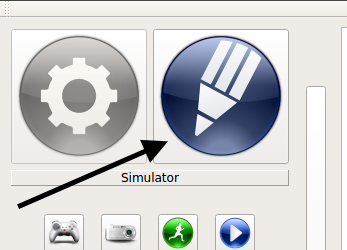
\includegraphics[width=0.5\textwidth,height=\textheight]{TutorialFigures/editorbutton.*}
\caption{The editor button}
\end{figure}

In the editor, you can place robot components together to build your
very own robot! Let's start by adding a circular body...

\begin{figure}
\centering
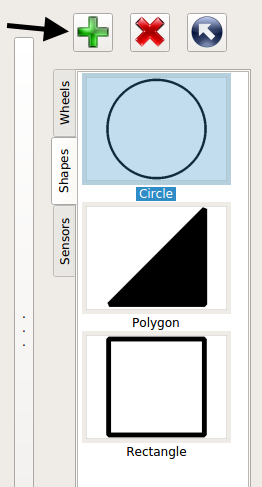
\includegraphics[width=0.5\textwidth,height=\textheight]{TutorialFigures/addcircle.*}
\caption{To select the circle from the shapes tab, and press the green
plus to add it}
\end{figure}

Next, we'll add a couple of wheels...

\begin{figure}
\centering
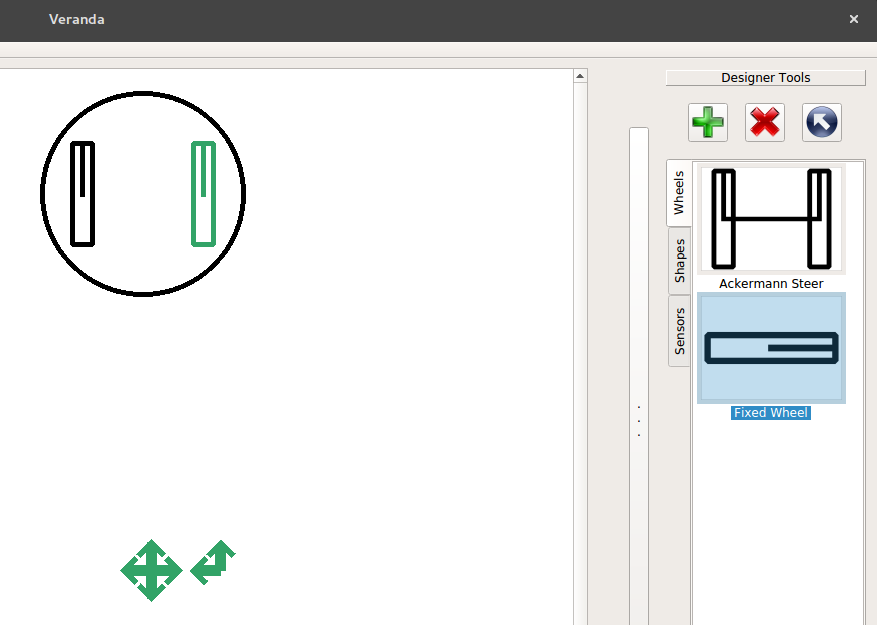
\includegraphics[width=0.75\textwidth,height=\textheight]{TutorialFigures/addwheels.*}
\caption{Completed turtle bot}
\end{figure}

Now, you may be noticing that my robot looks much more square than
yours; if you want to make sure the wheels are exactly where you want
them, you can set their position properties to the exact coordinates you
want. I made the wheels be exactly 0.6m to the left/right of the center,
and 0m above it.

\begin{figure}
\centering
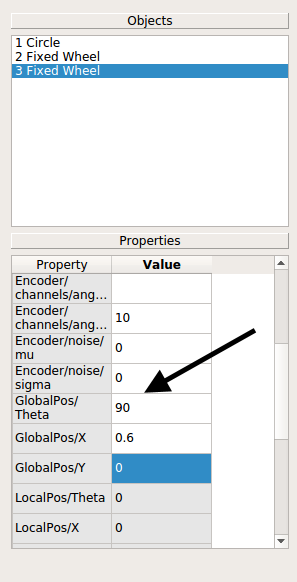
\includegraphics[width=0.5\textwidth,height=\textheight]{TutorialFigures/wheelproperties.*}
\caption{With a wheel selected, you can set properties for it}
\end{figure}

Now that you have a robot built, we need to load it into the simulation.
Choose the 'save' button, and save your robot as \texttt{Turtle.json}.
Don't forget the \texttt{.json}! It will not be added automatically if
you forget it.

\begin{figure}
\centering
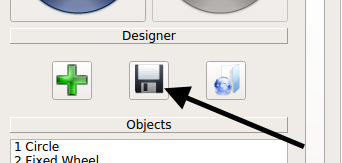
\includegraphics[width=0.5\textwidth,height=\textheight]{TutorialFigures/saverobot.*}
\caption{Save your robot by pressing the save button in the editor mode}
\end{figure}

Next we have to switch back to simulator mode.

\begin{figure}
\centering
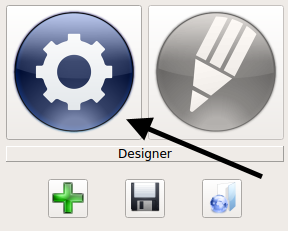
\includegraphics[width=0.5\textwidth,height=\textheight]{TutorialFigures/simulatorbutton.*}
\caption{The simulator button}
\end{figure}

Now, we can load the robot into our toolbox on the right.

\begin{figure}
\centering
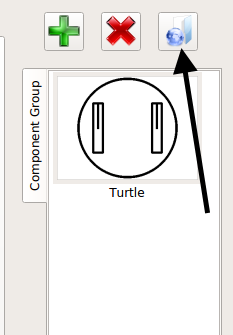
\includegraphics[width=0.5\textwidth,height=\textheight]{TutorialFigures/simulatorloadrobot.*}
\caption{Press the load button on the simulator toolbox to load a robot
file}
\end{figure}

And once your robot is in the toolbox, you can add it to the simulation
and position it wherever you want!

\begin{figure}
\centering
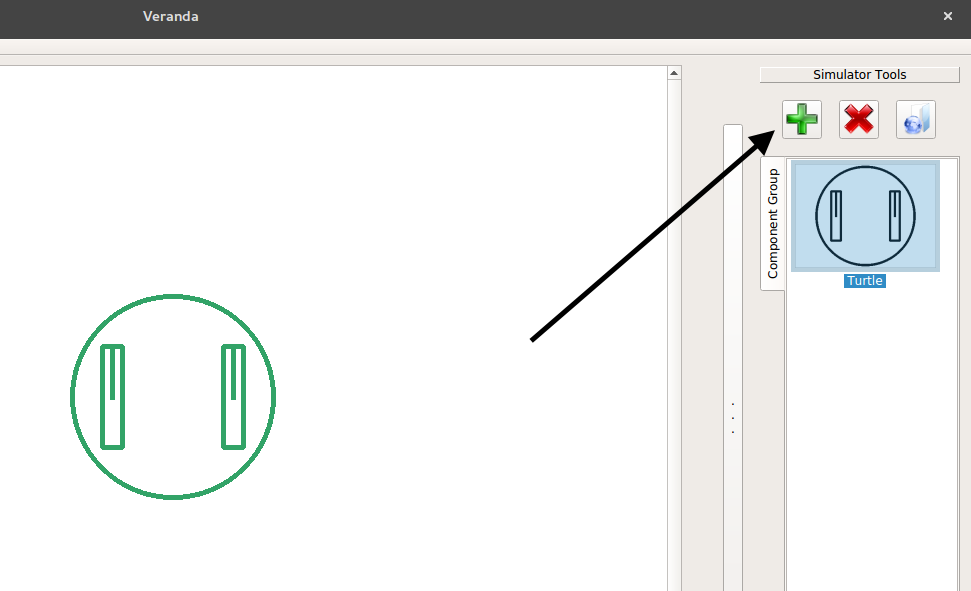
\includegraphics[width=0.75\textwidth,height=\textheight]{TutorialFigures/simulatoraddrobot.*}
\caption{Add robots from the toolbox by selecting them and pressing the
green plus}
\end{figure}

Finally, we can start the simulation with the 'play' button on the left.

\begin{figure}
\centering
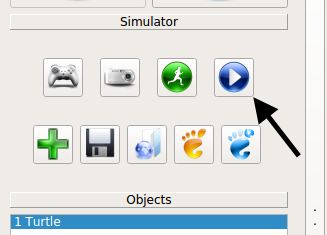
\includegraphics[width=0.5\textwidth,height=\textheight]{TutorialFigures/simulatorplaybutton.*}
\caption{The play button to start a simulation}
\end{figure}

Congratuations! You just simulated your first robot; it sat there, and
did nothing. Next, we're going to write some code to make it move.

Tip

If you don't want to go through the trouble of saving your robot in a
file and then loading it again, you can use the 'quick-add' button on
the editor to put it directly in the toolbox, but beware, if you close
Veranda, the robot will be lost forever!

\begin{figure}
\centering
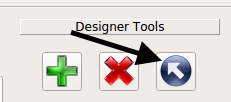
\includegraphics[width=0.5\textwidth,height=\textheight]{TutorialFigures/designerquickadd.*}
\caption{The designer quick-add button}
\end{figure}

\hypertarget{part-2-drive-your-robot-in-a-circle}{%
\subsection{Part 2: Drive your robot in a
circle}\label{part-2-drive-your-robot-in-a-circle}}

Now that we have a robot designed, we need to write some code to control
it and then connect that code to the simulation using ROS. First, we
will pick names for the ROS topics we want to use. Select your turtle
robot in the simulator, and then search through its properties for the
topic settings for the wheels. Since I left my wheels named 'Fixed
Wheel', I am looking for the properties called 'Fixed
Wheel1/channels/input\_speed', and 'Fixed Wheel2/channels/input\_speed'.
In my turtle, 'Fixed Wheel1' is on the left, and 'Fixed Wheel2' is on
the right, so I named the ROS topics 'robot0/left\_wheel' and
'robot0/right\_wheel', respectively.

\begin{figure}
\centering
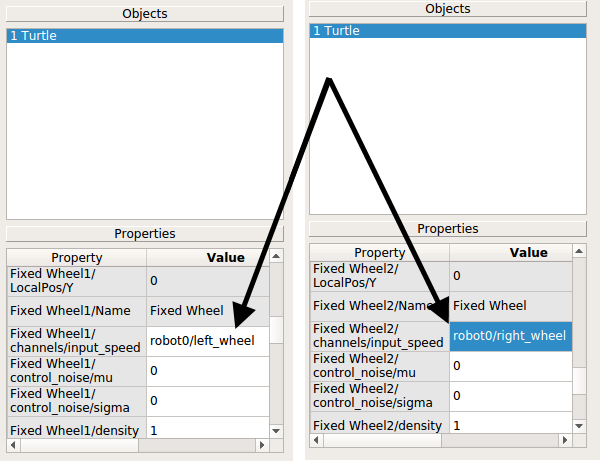
\includegraphics[width=0.75\textwidth,height=\textheight]{TutorialFigures/wheelchannels.*}
\caption{Setting the wheel control topics}
\end{figure}

We also need to indicate that the wheels can be driven. Find the
properties 'Fixed Wheel1/is\_driven' and Fixed Wheel2/is\_driven' and
set them both to be 'true'

Tip

Having issues telling your wheels apart? They have a 'Name' property
that can be changed in the editor to differentiate them better.

Tip

Don't want to have to set properties every time you start Veranda? You
can set many properties in the editor and save their values along with
the rest of the robot.

Now that the channels are set, we need to write some code to start
driving the robot. To drive a differential robot in a circle, all we
need to do is send a different speed command to each wheel; then they
will drive that speed forever.

First, we need our python to import the \texttt{rclpy} module, and the
Node type from that module

\begin{Shaded}
\begin{Highlighting}[]
\ImportTok{import}\NormalTok{ rclpy}
\ImportTok{from}\NormalTok{ rclpy.node }\ImportTok{import}\NormalTok{ Node}
\end{Highlighting}
\end{Shaded}

Next, we need to import the message type that should be used to
communicate to the wheels.

\begin{Shaded}
\begin{Highlighting}[]
\ImportTok{from}\NormalTok{ std\_msgs.msg }\ImportTok{import}\NormalTok{ Float32}
\end{Highlighting}
\end{Shaded}

Now, we can initialize ROS and create a Node to publish from

\begin{Shaded}
\begin{Highlighting}[]
\NormalTok{rclpy.init()}
\NormalTok{node }\OperatorTok{=}\NormalTok{ Node(}\StringTok{"circle"}\NormalTok{)}
\end{Highlighting}
\end{Shaded}

Once the node is created, we can create two publishers; one for each of
the wheel topics

\begin{Shaded}
\begin{Highlighting}[]
\NormalTok{publeft }\OperatorTok{=}\NormalTok{ node.create\_publisher(Float32, }\StringTok{\textquotesingle{}robot0/left\_wheel\textquotesingle{}}\NormalTok{)}
\NormalTok{pubright }\OperatorTok{=}\NormalTok{ node.create\_publisher(Float32, }\StringTok{\textquotesingle{}robot0/right\_wheel\textquotesingle{}}\NormalTok{)}
\end{Highlighting}
\end{Shaded}

Finally we can send a command to each of the wheels. Let's create a
Float32 message, and send it with different values to each wheel.

\begin{Shaded}
\begin{Highlighting}[]
\NormalTok{msg }\OperatorTok{=}\NormalTok{ Float32()}

\NormalTok{msg.data }\OperatorTok{=} \FloatTok{5.0}
\NormalTok{publeft.publish(msg)}

\NormalTok{msg.data }\OperatorTok{=} \FloatTok{10.0}
\NormalTok{pubright.publish(msg)}
\end{Highlighting}
\end{Shaded}

Note

This will command the wheels to drive 5 radians/second and 10
radians/second respectively.

However, if we run the code right now, the messages will not be sent;
they have only been queued for publishing. To send them out of the
application, we need to 'spin' the ROS node. Once we spin it, ROS will
enter an infinite loop which sends queued messages and receives incoming
ones.

\begin{Shaded}
\begin{Highlighting}[]
\NormalTok{rclpy.spin(node)}

\NormalTok{node.destroy\_node()}
\NormalTok{rclpy.shutdown()}
\end{Highlighting}
\end{Shaded}

And there we have it! One python program to start driving a robot in a
circle. Let's call it 'circle.py'

\begin{Shaded}
\begin{Highlighting}[]
\ImportTok{import}\NormalTok{ rclpy}
\ImportTok{from}\NormalTok{ rclpy.node }\ImportTok{import}\NormalTok{ Node}

\ImportTok{from}\NormalTok{ std\_msgs.msg }\ImportTok{import}\NormalTok{ Float32}

\NormalTok{rclpy.init()}
\NormalTok{node }\OperatorTok{=}\NormalTok{ Node(}\StringTok{"circle"}\NormalTok{)}

\NormalTok{publeft }\OperatorTok{=}\NormalTok{ node.create\_publisher(Float32, }\StringTok{\textquotesingle{}robot0/left\_wheel\textquotesingle{}}\NormalTok{)}
\NormalTok{pubright }\OperatorTok{=}\NormalTok{ node.create\_publisher(Float32, }\StringTok{\textquotesingle{}robot0/right\_wheel\textquotesingle{}}\NormalTok{)}

\NormalTok{msg }\OperatorTok{=}\NormalTok{ Float32()}

\NormalTok{msg.data }\OperatorTok{=} \FloatTok{5.0}
\NormalTok{publeft.publish(msg)}

\NormalTok{msg.data }\OperatorTok{=} \FloatTok{10.0}
\NormalTok{pubright.publish(msg)}

\NormalTok{rclpy.spin(node)}

\NormalTok{node.destroy\_node()}
\NormalTok{rclpy.shutdown()}
\end{Highlighting}
\end{Shaded}

Now, all that's left is to run it. First, we need to start the
simulation in Veranda because messages are not published or received
while the simulation is stopped. Once the simulation is running, we can
run our script to send a command to the wheels to start driving. This is
a three-command step, because we need to set up the ROS environment
first.

\begin{Shaded}
\begin{Highlighting}[]
\OperatorTok{\textgreater{}} \BuiltInTok{source}\NormalTok{ /opt/ros/ardent/setup.bash}
\OperatorTok{\textgreater{}} \BuiltInTok{source}\NormalTok{ \textasciitilde{}/veranda/local\_setup.bash}
\OperatorTok{\textgreater{}} \BuiltInTok{export} \VariableTok{RMW\_IMPLEMENTATION=}\NormalTok{rmw\_opensplice\_cpp}
\OperatorTok{\textgreater{}} \ExtensionTok{python3}\NormalTok{ circle.py}
\end{Highlighting}
\end{Shaded}

If all has gone well, the robot in your simulation will now be driving
in a circle! Your code will be in an infinite loop waiting to send and
receive messages, you can stop it with \texttt{Ctrl-C}

Tip

You don't need to do the two \texttt{source\ {[}path{]}} commands and
the \texttt{export\ RMW\_IMPLEMENTATION} every time you run your code,
just the first time. After you have sourced the environment for a
specific terminal, those environment variables will stay set up!

Important

Your robot might look a little goofy driving this circle. That's because
of the way the simulation handles relative mass; the body of the robot
is much larger than the wheels, so the wheels have a difficult time
moving it. Both wheels have a {density} property that you can use to
give them more oomph; I've found that setting the density of the wheels
in this demo robot to 5 works well. When you are building your own
robot, this is something you will have to adjust so that it drives
correctly.

Tip

Want to reset the simulation? Instead of removing the robot and putting
it in again, you can use the quicksave before starting the simulation
and quickload to reset to the saved version.

\begin{figure}
\centering

\includegraphics[width=0.25\textwidth,height=\textheight]{TutorialFigures/quicksaveload.*}
\caption{Quicksave (left) and Quickload (right)}
\end{figure}

\hypertarget{part-3-drive-a-more-complex-path}{%
\subsection{Part 3: Drive a more complex
path}\label{part-3-drive-a-more-complex-path}}

Driving in a circle is easy, but what if we want to make the robot drive
along some path that requires changing wheel speeds? Lets make it drive
a wiggle; first driving one wheel, then the other.

Once we call \texttt{rclpy.spin()}, our program goes into a loop, so how
do we send more commands? We use Timers with callbacks. A Timer in ROS
can be created to call a specific function every X seconds.

This is done with the function
\texttt{node.create\_timer(seconds,\ callback)}. The call returns a
Timer Handle, which can be used later to cancel the timer with
\texttt{node.destroy\_timer(handle)}.

So, let's set up some functions to drive a wiggle, they will both work
the same way, but one will drive the left wheel, and the other will
drive the right.

After we have created our \texttt{publeft} and \texttt{pubright}
publishers, we'll define our function

\begin{Shaded}
\begin{Highlighting}[]
\KeywordTok{def}\NormalTok{ wiggle\_left():}
\NormalTok{    msg }\OperatorTok{=}\NormalTok{ Float32()}

\NormalTok{    msg.data }\OperatorTok{=} \FloatTok{5.0}
\NormalTok{    publeft.publish(msg)}

\NormalTok{    msg.data }\OperatorTok{=} \FloatTok{0.0}
\NormalTok{    pubright.publish(msg)}
\end{Highlighting}
\end{Shaded}

This will stop the right wheel, and start the left wheel. Once we do
that, we need to start a timer. When the timer ends, we should call
\texttt{wiggle\_right} to stop the left wheel and start the right one.

\begin{Shaded}
\begin{Highlighting}[]
\KeywordTok{def}\NormalTok{ wiggle\_left():}
\NormalTok{    msg }\OperatorTok{=}\NormalTok{ Float32()}

\NormalTok{    msg.data }\OperatorTok{=} \FloatTok{5.0}
\NormalTok{    publeft.publish(msg)}

\NormalTok{    msg.data }\OperatorTok{=} \FloatTok{0.0}
\NormalTok{    pubright.publish(msg)}

\NormalTok{    node.create\_timer(}\DecValTok{1}\NormalTok{, wiggle\_right)}
\end{Highlighting}
\end{Shaded}

This will have a 1 second gap between commands. But wait! Timers in ROS
go for forever, so if we do this, we'll end up with a bunch of timers
starting and stopping the wheels, so we need to save the timer handle,
and be able to destroy the timer after it goes off.

\begin{Shaded}
\begin{Highlighting}[]
\KeywordTok{def}\NormalTok{ wiggle\_left():}
    \KeywordTok{global}\NormalTok{ timer\_handle}
\NormalTok{    node.destroy\_timer(timer\_handle)}

\NormalTok{    msg }\OperatorTok{=}\NormalTok{ Float32()}

\NormalTok{    msg.data }\OperatorTok{=} \FloatTok{5.0}
\NormalTok{    publeft.publish(msg)}

\NormalTok{    msg.data }\OperatorTok{=} \FloatTok{0.0}
\NormalTok{    pubright.publish(msg)}

\NormalTok{    timer\_handle }\OperatorTok{=}\NormalTok{ node.create\_timer(}\DecValTok{1}\NormalTok{, wiggle\_right)}
\end{Highlighting}
\end{Shaded}

If we do the same thing in the \texttt{wiggle\_right} function, then
they can share the timer handle and pass it between themselves. Finally,
we need to start the first timer before we spin the node.

\begin{Shaded}
\begin{Highlighting}[]
\NormalTok{timer\_handle }\OperatorTok{=}\NormalTok{ node.create\_timer(}\FloatTok{0.1}\NormalTok{, wiggle\_left)}
\NormalTok{rclpy.spin(node)}
\end{Highlighting}
\end{Shaded}

And there we have it! Now \texttt{wiggle.py} will drive the wheels
alternately. Go ahead and run it to see what it looks like.

\begin{Shaded}
\begin{Highlighting}[]
\ImportTok{import}\NormalTok{ rclpy}
\ImportTok{from}\NormalTok{ rclpy.node }\ImportTok{import}\NormalTok{ Node}

\ImportTok{from}\NormalTok{ std\_msgs.msg }\ImportTok{import}\NormalTok{ Float32}

\NormalTok{rclpy.init()}
\NormalTok{node }\OperatorTok{=}\NormalTok{ Node(}\StringTok{"wiggle"}\NormalTok{)}

\NormalTok{publeft }\OperatorTok{=}\NormalTok{ node.create\_publisher(Float32, }\StringTok{\textquotesingle{}robot0/left\_wheel\textquotesingle{}}\NormalTok{)}
\NormalTok{pubright }\OperatorTok{=}\NormalTok{ node.create\_publisher(Float32, }\StringTok{\textquotesingle{}robot0/right\_wheel\textquotesingle{}}\NormalTok{)}

\KeywordTok{def}\NormalTok{ wiggle\_left():}
    \KeywordTok{global}\NormalTok{ timer\_handle}
\NormalTok{    node.destroy\_timer(timer\_handle)}

\NormalTok{    msg }\OperatorTok{=}\NormalTok{ Float32()}

\NormalTok{    msg.data }\OperatorTok{=} \FloatTok{5.0}
\NormalTok{    publeft.publish(msg)}

\NormalTok{    msg.data }\OperatorTok{=} \FloatTok{0.0}
\NormalTok{    pubright.publish(msg)}

\NormalTok{    timer\_handle }\OperatorTok{=}\NormalTok{ node.create\_timer(}\DecValTok{1}\NormalTok{, wiggle\_right)}

\KeywordTok{def}\NormalTok{ wiggle\_right():}
    \KeywordTok{global}\NormalTok{ timer\_handle}
\NormalTok{    node.destroy\_timer(timer\_handle)}

\NormalTok{    msg }\OperatorTok{=}\NormalTok{ Float32()}

\NormalTok{    msg.data }\OperatorTok{=} \FloatTok{0.0}
\NormalTok{    publeft.publish(msg)}

\NormalTok{    msg.data }\OperatorTok{=} \FloatTok{5.0}
\NormalTok{    pubright.publish(msg)}

\NormalTok{    timer\_handle }\OperatorTok{=}\NormalTok{ node.create\_timer(}\DecValTok{1}\NormalTok{, wiggle\_left)}

\NormalTok{timer\_handle }\OperatorTok{=}\NormalTok{ node.create\_timer(}\FloatTok{0.1}\NormalTok{, wiggle\_left)}
\NormalTok{rclpy.spin(node)}

\NormalTok{node.destroy\_node()}
\NormalTok{rclpy.shutdown()}
\end{Highlighting}
\end{Shaded}

\hypertarget{part-4-hooking-into-the-simulation-clock}{%
\subsection{Part 4: Hooking into the Simulation
Clock}\label{part-4-hooking-into-the-simulation-clock}}

Now that you have a couple of scripts running, let's take a look at what
happens when we use the time-warp capabilities of Veranda. Click the
time-warp button while your \texttt{wiggle.py} is driving a robot.

\begin{figure}
\centering
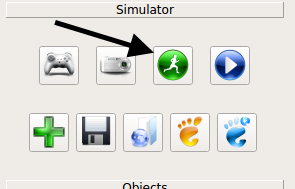
\includegraphics[width=0.5\textwidth,height=\textheight]{TutorialFigures/timewarpbutton.*}
\caption{The time warp button; press it multiple times to cycle through
2x, 3x, and 0.5x speeds}
\end{figure}

That probably didn't do what you expected, did it? The issue here is
that, in the simulation, time started moving faster, but the clock in
your control script didn't! So for every 1 second of wiggling that the
control code thought it was doing, the simulator was actually driving
the robot for more than 1 second.

This can be accounted for by using the Veranda SimTimer. The SimTimer
listens to the clock message coming from Veranda, and uses those to
determine how much time has passed, instead of the sytem clock.

First, we need to include the SimTimer module

\begin{Shaded}
\begin{Highlighting}[]
\ImportTok{from}\NormalTok{ veranda.SimTimer }\ImportTok{import}\NormalTok{ SimTimer}
\end{Highlighting}
\end{Shaded}

Next, after we create our ROS node, we create a timer object which uses
that node.

\begin{Shaded}
\begin{Highlighting}[]
\NormalTok{simTime }\OperatorTok{=}\NormalTok{ SimTimer(}\VariableTok{True}\NormalTok{, }\StringTok{"veranda/timestamp"}\NormalTok{, node)}
\end{Highlighting}
\end{Shaded}

Note

\begin{description}
\item[The parameters for the SimTimer are]
\begin{itemize}
\tightlist
\item
  Boolean - Should it use the Simulation Timer? If False, the regular
  system clock is used
\item
  String - ROS Topic that the timestamp is published to. This is
  currently always the same
\item
  Node - The ROS Node that should be used to listen for time messages
\end{itemize}
\end{description}

Now, everywhere that we have \texttt{node.create\_timer} and
\texttt{node.destroy\_timer}, we can replace with
\texttt{simTime.create\_timer} and \texttt{simTime.destroy\_timer}. It's
that easy! Go ahead and run your new wiggle code, and test out how it
works with the time-warp feature.

Important

While the create and destroy functions behave similarly, the SimTimer
does not return the same dataType as the ROS Node. If the SimTimer is
using the timestamp message, it will return integer values as the timer
handles, but if it is using the regular ROS timer functionality, (Param
1 is False), it will return the Timer type that
\texttt{Node.create\_timer()} yields.

\begin{Shaded}
\begin{Highlighting}[]
\ImportTok{import}\NormalTok{ rclpy}
\ImportTok{from}\NormalTok{ rclpy.node }\ImportTok{import}\NormalTok{ Node}

\ImportTok{from}\NormalTok{ std\_msgs.msg }\ImportTok{import}\NormalTok{ Float32}

\ImportTok{from}\NormalTok{ veranda.SimTimer }\ImportTok{import}\NormalTok{ SimTimer}

\NormalTok{rclpy.init()}
\NormalTok{node }\OperatorTok{=}\NormalTok{ Node(}\StringTok{"wiggle"}\NormalTok{)}

\NormalTok{simTime }\OperatorTok{=}\NormalTok{ SimTimer(}\VariableTok{True}\NormalTok{, }\StringTok{"veranda/timestamp"}\NormalTok{, node)}

\NormalTok{publeft }\OperatorTok{=}\NormalTok{ node.create\_publisher(Float32, }\StringTok{\textquotesingle{}robot0/left\_wheel\textquotesingle{}}\NormalTok{)}
\NormalTok{pubright }\OperatorTok{=}\NormalTok{ node.create\_publisher(Float32, }\StringTok{\textquotesingle{}robot0/right\_wheel\textquotesingle{}}\NormalTok{)}

\KeywordTok{def}\NormalTok{ wiggle\_left():}
    \KeywordTok{global}\NormalTok{ timer\_handle}
\NormalTok{    simTime.destroy\_timer(timer\_handle)}

\NormalTok{    msg }\OperatorTok{=}\NormalTok{ Float32()}

\NormalTok{    msg.data }\OperatorTok{=} \FloatTok{5.0}
\NormalTok{    publeft.publish(msg)}

\NormalTok{    msg.data }\OperatorTok{=} \FloatTok{0.0}
\NormalTok{    pubright.publish(msg)}

\NormalTok{    timer\_handle }\OperatorTok{=}\NormalTok{ simTime.create\_timer(}\DecValTok{1}\NormalTok{, wiggle\_right)}

\KeywordTok{def}\NormalTok{ wiggle\_right():}
    \KeywordTok{global}\NormalTok{ timer\_handle}
\NormalTok{    simTime.destroy\_timer(timer\_handle)}

\NormalTok{    msg }\OperatorTok{=}\NormalTok{ Float32()}

\NormalTok{    msg.data }\OperatorTok{=} \FloatTok{0.0}
\NormalTok{    publeft.publish(msg)}

\NormalTok{    msg.data }\OperatorTok{=} \FloatTok{5.0}
\NormalTok{    pubright.publish(msg)}

\NormalTok{    timer\_handle }\OperatorTok{=}\NormalTok{ simTime.create\_timer(}\DecValTok{1}\NormalTok{, wiggle\_left)}

\NormalTok{timer\_handle }\OperatorTok{=}\NormalTok{ simTime.create\_timer(}\FloatTok{0.1}\NormalTok{, wiggle\_left)}
\NormalTok{rclpy.spin(node)}

\NormalTok{node.destroy\_node()}
\NormalTok{rclpy.shutdown()}
\end{Highlighting}
\end{Shaded}
